\documentclass{bmd2016p}

\begin{document}

\begin{center}
\fontsize{14}{20}{\bf Buckling and dynamic collapse of the bicycle wheel}
\end{center}

%%%%%%%%%%%%%%%% authors %%%%%%%%%%%%%%%
\begin{center}
\normalsize{\bf{M. Ford$^{*}$, J.M. Papadopoulos$^\#$, 
            O. Balogun$^\dag$}}
\end{center} 

\begin{center}
\begin{tabular}{c}
$^*$ Department of Mechanical Engineering\\
Northwestern University\\
2145 Sheridan Road, Evanston, IL 60208, USA\\
e-mail: mford@u.northwestern.edu\\[2.5ex]

$^\#$ Department of Mechanical and Industrial Engineering\\
Northeastern University\\
360 Huntington Ave., Boston, MA 02115, USA\\
e-mail: j.papadopoulos@neu.edu\\[2.5ex]

$^\dag$ Department of Civil Engineering\\
Northwestern University\\
2145 Sheridan Road, Evanston, IL 60208, USA\\
e-mail: o.balogun@northwestern.edu\\
\end{tabular}
\end{center}


\section*{ABSTRACT}

The first page begins with the title of the paper, the authors, affiliations, 
abstract and keywords as it is shown in this document. The title of the paper 
should be typed in 14\,pt bold font and be centred. It should be separated 
from the symposium name by a 12\,pt space and from authors' names by an 18\,pt 
space. Authors' names should be typed in bold font. Affiliations should be 
typed in a general formatting style, centred within a corresponding bounding 
box. The abstract part of the final paper should not be longer than about 
300~words, so it fits on the title page. The abstract begins with the 
``ABSTRACT'' header typed in bold 11\,pt font. The abstract text should be 
separated from the header by an 11\,pt space. The abstract should be followed 
by a list of keywords after the header ``Keywords:'' typed in bold 11\,pt 
font. The keywords should be separated by commas. A dot should be place after 
the last keyword. Up to about five keywords are allowed. Title, affiliations, 
abstract and keywords have to fit on the title page. The Introduction 
paragraph may start already on the title page provided there is enough space.

\begin{keywords}
bicycle wheel, 
buckling, 
bifurcation.
\end{keywords}

\section{INTRODUCTION}

The bicycle wheel is a prestressed structure and is susceptible to buckling under internal forces. As the spokes are tightened uniformly, the rim deforms radially to accommodate the spoke strain. At a critical tension, the system reaches a bifurcation point and the rim buckles out of its initial plane. The post-buckling configuration is generally stable and the original shape of the wheel can be recovered by reducing the tension. Buckling can also be triggered by external forces in an otherwise stable wheel leading to a release of strain energy. This is an unstable process which generally leads to catastrophic failure.

Despite its implications for wheel strength, the buckling problem has never received a rigorous treatment to our knowledge. Jobst Brandt alludes to buckling in his practical manual for wheelbuilders\cite{Brandt1993c}:

``If the wheel becomes untrue in two large waves during stress relieving, the maximum, safe tension has been exceeded. Approach this tension carefully to avoid major rim distortions. When the wheel loses alignment from stress relieving, loosen all spokes a half turn before retruing the wheel.''

He did not discuss the problem further, but suggested that wheel failure commonly occurs due to a loss of lateral stability caused by spoke buckling. Pippard and Francis\cite{Pippard1932d} derived a model for lateral stiffness based on the elastic foundation model, but did not discuss stability and neglected any effects of spoke tension.

Flexural-torsional buckling of rings can be treated as a special case of buckling of arches, where the included angle is allowed to go to $2\pi$. Timoshenko and Gere\cite{Timoshenko1961a} gave a formula for the critical load for a ring with doubly-symmetric cross-section subjected to radial loads. The theory of flexural-torsional buckling of monosymmetric arches (bicycle rims have only one plane of symmetry) was broadly formalized by Trahair and Papangelis\cite{Trahair1987b} using the virtual work approach to derive the equilibrium and stability equations. Their theory has been extended to treat arches restrained by continuous\cite{Pi2002b} or discrete\cite{Bradford2002d} elastic supports and elastic end restraints\cite{Guo2014b}.

The problem of the prestressed bicycle wheel is unique for a number of reasons. First, the buckling load is internal to the structure. Second, the spokes act both as elastic restraints resisting buckling and as prestressing elements causing buckling. Third, the lateral, radial, and torsional restraining actions of the spokes are coupled---i.e. lateral deflection at a spoke may produce lateral, radial, and torsional reactions. These considerations extend to other structural systems. Large observation wheels such as the London Eye\cite{Mann2001a} and the Singapore Flyer\cite{Allsop2009a} resemble large bicycle wheels and achieve lateral stability due to the bracing angle of prestressed cables, and must be designed against flexural-torsional buckling.

Here we derive a general theory for buckling of a spoked bicycle wheel under self-tension and investigate several special cases. Furthermore, we analyze large deformation post-buckling behavior and show how local buckling of individual spokes can lead to collapse of an otherwise sub-critical wheel.


\section{GENERAL INSTRUCTIONS}

The paper must be written in English. It must contain the full name, address 
and e-mail address of each author. No hard limits on the total length of the 
paper are set, but it should better not exceed 20 pages. All page margins 
should be 3\,cm. The paper used should have the size 210\,x\,297\, mm 
which is the European (German) A4 size. It is suggested to use styles for 
formatting and automatic reference, figure numbering to avoid editorial 
errors. To avoid compatibility problems it is advised to use only upper or 
lower case Latin alphabet, numbers and the underscore character in the file 
name.


\subsection{Equations}

Equations should be numbered continuously according to the format shown in 
Equation~(\ref{eq:equ1}): 
\begin{equation} \label{eq:equ1}
  e^{i\pi} + 1 = 0, 
\end{equation}
where the unknown symbols are explained after the equation.


\subsection{Figures and tables}

\begin{table}[h!]
\begin{center}
\caption{Example of a table with a short caption.} \label{tab:tab1}
\begin{tabular}{|c|ccc|}
\hline
    &  $x$  &  $y$  &  $z$ \\
\hline
$x'$  &  $\alpha_1$ & $\beta_1$ & $\gamma_1$ \\
$y'$  &  $\alpha_2$ & $\beta_2$ & $\gamma_2$ \\
$z'$  &  $\alpha_3$ & $\beta_3$ & $\gamma_3$ \\
\hline
\end{tabular}
\end{center}
\end{table}
All figures should be clearly readable and relevant to the presented text. Use 
of at least 300\,dpi resolution for pictures and 600\,dpi for line art is 
required, 1\,px wide lines in figures should be avoided as they may become 
invisible in print. There is no limit on the amount of figures as long as they 
do not dominate the text and the total length of the paper is within the 
specified limits. Both figures and tables should be centred on the page.

\begin{figure}[h!]
\begin{center}
  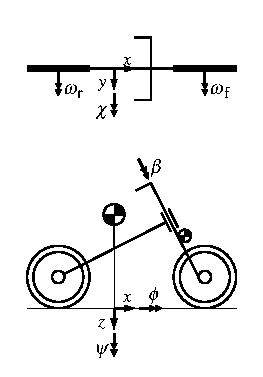
\includegraphics[width=55mm]{figure1}
  \caption{An example of a figure caption. Use 10~pt Times New Roman.
           For long captions, use a text width of 13~cm.
           Use the same style for the tables.} \label{fig:fig1}
\end{center}
\end{figure}
Figures, graphs and tables must be included in the same style as shown for 
Figure~\ref{fig:fig1} and Table~\ref{tab:tab1}.


\subsection{References}

Bibliographical citations should be written in the order in which they are 
cited, see the References section below, where Reference~\cite{Pac02} 
exemplifies the case of a textbook, while Reference~\cite{Ber07} is an article 
in conference proceedings and Reference~\cite{Sha71} is an article in a 
journal. Use can be made of a pre-existing bibtex style which uses a similar 
style.


\section{SUBMISSION OF PAPER}

The paper should be submitted by e-mail to \href{mailto:jbrendelson@bmd2016mke.org}{jbrendelson@bmd2016mke.org} with the email subject containing the phrase \textit{``BMD 2016 paper submission - submitting author last name''}. \uline{The deadline is September 1st, 2016}. The file of the paper must be in the Portable Document Format (PDF) and the file size should be within the limit of 10 MB. Exceptionally, other file formats can be accepted if the symposium organizers have been informed beforehand. 

Please make sure that the final version of the paper complies with the standards set here. Please note slightly different formatting requirements of the abstract and the final paper.

\section{CONCLUSIONS}

We very much look forward to welcoming you in Milwaukee! Best wishes and the 
warmest regards from the Organizing Committee of Bicycle and Motorcycle 
Dynamics 2016.

\bibliographystyle{acm}
\bibliography{C:/Users/matt/OneDrive/Documents/Research/bibtex/Papers-BMD2016.bib}

\end{document}
